\begin{section}{Relations}

While there is no agreed upon universal definition of mathematics, one could argue that mathematics focuses on the study of patterns and relationships. Certain types of relationships occur over and over in mathematics.  One way of formalizing the abstract nature and structure of these relationships is with the notion of \emph{relations}. In Chapter~\ref{chap:Functions}, we will see that a function is a special type of relation.

Recall from Section~\ref{sec:Cartesian Products} that the Cartesian product of two sets $A$ and $B$, written $A\times B$, is the set of all ordered pairs $(a,b)$, where $a\in A$ and $b\in B$. That is, $A\times B=\{(a,b)\mid a\in A, b\in B\}$.

\begin{definition}
Let $A$ and $B$ be sets. A \textbf{relation $R$ from $A$ to $B$} is a subset of $A \times B$. If $R$ is a relation from $A$ to $B$ and $(a,b)\in {R}$, then we say that \textbf{$a$ is related to $b$} and we may write $aR b$ in place of $(a,b)\in{R}$. If $R$ is a relation from $A$ to the same set $A$, then we say that $R$ is a \textbf{relation on $A$}.
\end{definition}

\begin{example}
The set $\mathbb{N}\times \mathbb{R}$ from Problem~\ref{prob:some lines} is an example of a relation on $\mathbb{R}$ since $\mathbb{N}\times \mathbb{R}$ is a subset of $\mathbb{R}\times \mathbb{R}$.
\end{example}

It is important to notice that the order in which we write things for relations matters.  In particular, if $R$ is a relation from $A$ to $B$ and $a R b$, then it may or may not be the case that $bR a$.

\begin{example}\label{ex:relation finite to finite}
If $A=\{a,b,c,d,e\}$ and $B=\{1,2,3,4\}$, then the set of ordered pairs
\[
R=\{(a,1),(a,2),(a,4),(c,2),(d,2),(e,2),(e,4)\}
\]
is an example of a relation from $A$ to $B$. In this case, we could write $(c,2)\in{R}$ or $cR 2$. We could also say that $a$ is related to 1, 2, and 4. 
\end{example}

\begin{example}\label{ex:relation on finite}
As in the previous example, let $A=\{a,b,c,d,e\}$. One possible relation on $A$ is given by
\[
R=\{(a,a),(a,b),(a,c),(b,b),(b,a),(b,c),(c,d),(c,e),(d,d),(d,a),(d,c),(e,a)\}.
\]
\end{example}

\begin{example}\label{ex:Twitter}
Consider the set of accounts $A$ on the social media platform Twitter.  On Twitter, each account has a set of accounts that they follow.  We can model this situation mathematically using a relation on $A$.  Define $T$ on $A$ via $xTy$ if and only if $x$ follows $y$ on Twitter. As a set
\[
T=\{(x,y)\in A\times A\mid x\text{ follows }y\text{ on Twitter}\}.
\]
\end{example}

\begin{example}
You are already familiar with many relations.  For example, $=$, $\leq$, and $<$ are each examples of relations on the real numbers. We could say that $(3,\pi)$ is in the relation $\leq$ and the relation $<$ since $3\leq \pi$ and $3<\pi$.  However, $(3,\pi)$ is not in the relation $=$ since $3\neq \pi$.  Also, notice that order matters for the relations $\leq$ and $<$ yet does not for $=$. For example, $(-\sqrt{2}, 4)$ is in the relation $\leq$ while $(4,-\sqrt{2})$ is not.
\end{example}

%\begin{example}
%Let $P$ denote the set of all people. Define $\mapsto$ on $P$ via $x\mapsto y$ if and only if $x$ is friends with $y$.  Then $\mapsto$ is a relation on $P$.
%\end{example}

\begin{example}
Define the relation $S$ from $\{-1,1\}$ to $\mathbb{Z}$ via $1Sx$ if and only if $x$ is even and $-1Sx$ if and only if $x$ is odd.  That is, $1$ is related to all even integers and $-1$ is related to all odd integers.
\end{example}

\begin{example}
Let $A$ be any set.  Since $\emptyset \subseteq A\times A$, the empty set forms a relation on $A$. This relation is called the \textbf{empty relation} on $A$.
\end{example}

Relations can be represented using digraphs. A \textbf{digraph} (short for \emph{directed graph}) is a discrete graph that consists of a set of vertices connected by edges, where the edges have a direction associated with them. If $R$ is a relation from $A$ to $B$, then the elements of $A$ and $B$ are the vertices of the digraph and there is a directed edge from $a\in A$ to $b\in B$ if and only if $(a,b)$ is in the relation $R$ (i.e., $aR b$). We can visually represent digraphs by using dots to represent the vertices and arrows to represent directed edges. We will not make a distinction between a digraph and its visual representation. Utilizing a digraph to represent a relation may be impractical if there is a large number of vertices or directed edges. 

\begin{example}
Consider the relation given in Example~\ref{ex:relation finite to finite}.  The corresponding digraph is depicted in Figure~\ref{fig:digraph finite to finite}. Notice that we have placed the vertices corresponding to elements of $A$ on the left and the elements of $B$ on the right.  This is standard practice, but what really matters is the edge connections not how the vertices are placed on the page.
\end{example}

\tikzset{every loop/.style={min distance=8mm}}
\tikzstyle{vert} = [circle, draw, fill=grey,inner sep=0pt, minimum size=5mm]
\tikzstyle{b} = [draw,-stealth]

\begin{figure}[h!]
\begin{center}
\begin{tikzpicture}[->,>=stealth,shorten >=1pt,auto,node distance=2cm,semithick,scale=1.2]

\node[vert] (A) at (0,5) {\scriptsize $a$};
\node[vert] (B) at (0,4) {\scriptsize $b$};
\node[vert] (C) at (0,3) {\scriptsize $c$};
\node[vert] (D) at (0,2) {\scriptsize $d$};
\node[vert] (E) at (0,1) {\scriptsize $e$};

\node[vert] (1) at (2.5,4.5) {\scriptsize $1$};
\node[vert] (2) at (2.5,3.5) {\scriptsize $2$};
\node[vert] (3) at (2.5,2.5) {\scriptsize $3$};
\node[vert] (4) at (2.5,1.5) {\scriptsize $4$};

\path (A) edge node {} (1)
(A) edge node {} (2)
(A) edge node {} (4)
(C) edge node {} (2)
(D) edge node {} (2)
(E) edge node {} (2)
(E) edge node {} (4);

\node[draw,fit=(A) (B) (C) (D) (E),minimum width=1.5cm,gray] {};
\node[draw,fit=(1) (2) (3) (4),minimum width=1.5cm,gray] {};
\node at (0,5.7) {$A$};
\node at (2.5,5.2) {$B$}; 
\end{tikzpicture}
\caption{Digraph for a relation from $A=\{a,b,c,d,e\}$ to $B=\{1,2,3,4\}$.}\label{fig:digraph finite to finite}
\end{center}
\end{figure}

\begin{problem}
Let $A=\{1,2,3,4,5,6\}$ and $B=\{1,2,3,4\}$ and define $D$ from $A$ to $B$ via $(a,b)\in D$ if and only if $a-b$ is divisible by 2.  List the ordered pairs in $D$ and draw the corresponding digraph.
\end{problem}

If $R$ is a relation on $A$ (i.e., a relation from $A$ to $A$), then we can simplify the structure of the digraph by only utilizing one copy of $A$ for the vertices. In this case, we may have directed edges that point from a vertex to itself.  When drawing digraphs for a relation on a set, we will default to this simplified digraph (like the one depicted in Figure~\ref{fig:digraph on finite}\subref{fig:digraphB}).

\begin{example}\label{ex:digraph}
Figure~\ref{fig:digraph on finite}\subref{fig:digraphA} represents the relation of Example~\ref{ex:relation on finite} as a digraph from $A$ to $A$ while the digraph in Figure~\ref{fig:digraph on finite}\subref{fig:digraphB} provides a streamlined representation of the same relation that uses the elements in $A$ only once instead of twice.
\end{example}

\begin{figure}[h!]
\centering
\subcaptionbox{\label{fig:digraphA}}[.48\linewidth]{
\begin{tikzpicture}[->,>=stealth,shorten >=1pt,auto,node distance=2cm,semithick,scale=1.2]

\node[vert] (A1) at (0,5) {\scriptsize $a$};
\node[vert] (B1) at (0,4) {\scriptsize $b$};
\node[vert] (C1) at (0,3) {\scriptsize $c$};
\node[vert] (D1) at (0,2) {\scriptsize $d$};
\node[vert] (E1) at (0,1) {\scriptsize $e$};

\node[vert] (A2) at (2.5,5) {\scriptsize $a$};
\node[vert] (B2) at (2.5,4) {\scriptsize $b$};
\node[vert] (C2) at (2.5,3) {\scriptsize $c$};
\node[vert] (D2) at (2.5,2) {\scriptsize $d$};
\node[vert] (E2) at (2.5,1) {\scriptsize $e$};

\path (A1) edge node {} (A2)
(A1) edge node {} (C2)
(A1) edge node {} (B2)
(B1) edge node {} (B2)
(B1) edge node {} (A2)
(B1) edge node {} (C2)
(C1) edge node {} (D2)
(C1) edge node {} (E2)
(D1) edge node {} (D2)
(D1) edge node {} (A2)
(D1) edge node {} (C2)
(E1) edge node {} (A2);

\node[draw,fit=(A1) (B1) (C1) (D1) (E1),minimum width=1.5cm,gray] {};
\node[draw,fit=(A2) (B2) (C2) (D2) (E2),minimum width=1.5cm,gray] {};
\node at (0,5.7) {$A$};
\node at (2.5,5.7) {$A$};
\end{tikzpicture}
}
\subcaptionbox{\label{fig:digraphB}}[.48\linewidth]{
\begin{tikzpicture}[->,>=stealth,shorten >=1pt,auto,node distance=2cm,semithick]

\node[vert] (A)                    {\scriptsize $a$};
\node[vert] (B) [above right of=A] {\scriptsize $b$};
\node[vert] (D) [below right of=A] {\scriptsize $d$};
\node[vert] (C) [below right of=B] {\scriptsize $c$};
\node[vert] (E) [below of=D]       {\scriptsize $e$};

\path (B) edge [bend left]  node {} (A)
(A) edge [bend left]  node {} (B)
            edge              node {} (C)
(B) edge [out=135,in=45,loop] node {} (B)
    edge [bend left]  node {} (C)
(D) edge [bend left]  node {} (C)
(C) edge [bend left]  node {} (D)
    edge [bend left]  node {} (E)
(A) edge [out=-135,in=135,loop]  node {} (A)
(D) edge [out=-45, in=-135,loop] node {} (D)
    edge [bend left]  node {} (A)
(E) edge [bend left]  node {} (A)
(C) edge [out=45, in=-45,loop,white] node {} (C);
\end{tikzpicture}
}
\caption{Two variations of digraphs for a relation on $A=\{a,b,c,d,e\}$.}\label{fig:digraph on finite}
\end{figure}

\begin{problem}\label{prob:divides}
Let $A=\{1,2,3,4,5,6\}$ and define $|$ on $A$ via $x|y$ if and only if $x$ divides $y$.  List the ordered pairs in $|$ and draw the corresponding digraph.
\end{problem}

\begin{problem}\label{prob:another relation on finite}
Let $A=\{a,b,c,d\}$ and define $R$ on $A$ via
\[
{R}=\{(a,a),(a,b),(a,c),(b,b),(b,a),(b,c),(c,c),(c,a),(c,b),(d,d)\}.
\]  
\begin{enumerate}[label=\textrm{(\alph*)}]
\item Draw the digraph for $R$.
\item Draw the digraph for the empty relation on $A$.
\end{enumerate}
\end{problem}

%Often it is not feasible to draw the complete diagram for the digraph of a relation (e.g., when the sets involved are infinite).  However, sometimes we can still provide a visual representation of the relation by plotting points that are in the relation. 

We can also visually represent a relation by plotting the points in the relation.  In particular, if $R$ is a relation from $A$ to $B$ and $aR b$, we can plot all points $(a,b)$ that satisfy $aR b$ in two dimensions, where we interpret the set $A$ to be the horizontal axis and $B$ to be the vertical axis. We will refer to this visual representation of a relation as the \textbf{graph} of the relation.%\footnote{Some mathematics texts do not make a distinction between a relation and the graph of a relation.}

\begin{example}\label{ex:circle}
When we write $x^2+y^2=1$, we are implicitly defining a relation.  In particular, the relation is the set of ordered pairs $(x,y)$ satisfying $x^2+y^2=1$, namely $\{(x,y)\in \mathbb{R}^2 \mid x^2+y^2=1\}$. The graph of this relation in $\mathbb{R}^2$ is the unit circle centered at the origin in the plane as shown in Figure~\ref{fig:unit circle}.
\end{example}

\begin{figure}[h!]
\centering
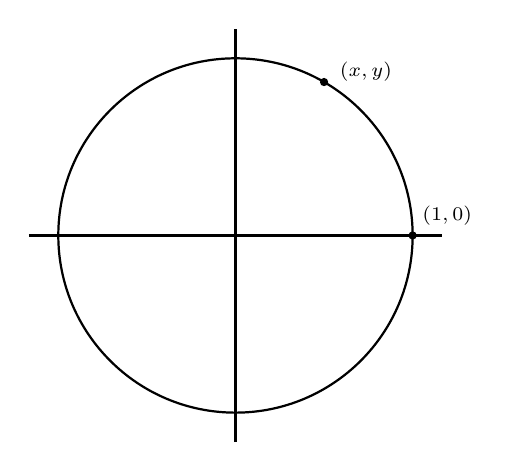
\begin{tikzpicture}[scale=.75,angle/.style={fill=white},point/.style={}]
\draw [thick,] (0,0) circle (3cm);
\draw [thick, ] (-3.5,0) -- (3.5,0);
\draw [thick, ] (0,-3.5) -- (0,3.5);
\fill (0:3) circle (0.07cm);
\node at (0:3) [above right] {\scriptsize $ (1,0) $};
\fill (60:3) circle (0.07cm);
\node at (60:3.2)[right=0.01ex] {\scriptsize $ (x,y) $};
\end{tikzpicture}
\caption{Graph of the relation determined by $x^2+y^2=1$.}\label{fig:unit circle}
\end{figure}

\begin{problem}\label{prob:parabola}
For each of the following, draw a portion of the graph that represents the relation as a subset of $\mathbb{R}^2$.
\begin{enumerate}[label=\textrm{(\alph*)}]
\item $\{(x,y)\in \mathbb{R}^2 \mid y=x^2\}$
\item $\{(x,y)\in \mathbb{Z}^2 \mid y=x^2\}$
\item $\{(x,y)\in \mathbb{R}^2 \mid y^2=x\}$
\item $\{(x,y)\in \mathbb{N}\times \mathbb{R} \mid y^2=x\}$
\end{enumerate}
\end{problem}

\begin{problem}
Draw a portion of the graph that represents the relation $\leq$ on $\mathbb{R}$.
\end{problem}

For a relation on a set, it is natural to consider the collection of elements that a given element is related to.  For example, a user's ``Following List" on Twitter is the set of accounts on Twitter that the user is following. %Be careful not to confuse ``Following List" with ``Followers List".  The latter is the set of accounts that follow a user.  

\begin{definition}\label{def:relatives}
Let $R$ be a relation on a set $A$. For each $a\in A$, we define the \textbf{set of relatives of $a$ with respect to $R$} via
\[
\boxed{\rel(a,R):=\{b\in A\mid aR b\}}.
\]
We also define the \textbf{collection of the sets of relatives with respect to $R$} by
\[
\boxed{\Rel(R):=\{\rel(a)\mid a\in A\}}.
\]
\end{definition}

If $R$ is clear from the context, we will usually write $\boxed{\rel(a)}$ in place of $\rel(a,R)$.  In terms of digraphs, $\rel(a)$ is the collection of vertices that have a directed edge pointing towards them from the vertex labeled by $a$. In graph theory, this collection of vertices is called the \textbf{out neighborhood} of $a$ and each such vertex is called an \textbf{out neighbor}. Notice that $\Rel(R)$ is a set of sets.  In particular, an element in $\Rel(R)$ is a subset of $A$---equivalently, an element of $\mathcal{P}(A)$.

\begin{example}
Consider the relation given in Example~\ref{ex:relation on finite}.  By inspecting the ordered pairs in $R$ or by looking at the digraph in Figure~\ref{fig:digraph on finite}\subref{fig:digraphB}, we see that
\[
\rel(a) = \{a,b,c\},\ \rel(b) = \{a,b,c\},\ \rel(c) = \{d,e\},\ \rel(d) = \{a,c,d\},\ \rel(e) = \{a\},
\]
so that $\Rel(R) = \{\{a,b,c\},\{d,e\},\{a,c,d\},\{a\}\}$.
\end{example}

\begin{problem}
Consider the relation given in Problem~\ref{prob:another relation on finite}(a).  Find $\Rel(R)$ by determining $\rel(x)$ for each $x\in A$.
\end{problem}

\begin{problem}
Describe the collection of the sets of relatives with respect to the empty relation from Problem~\ref{prob:another relation on finite}(b).
\end{problem}

\begin{problem}\label{prob:facebook}
Let $P$ denote the set of all people with accounts on Facebook and define the relation $F$ on $P$ via $xFy$ if and only if $x$ is friends with $y$. Describe $\rel(\text{Maria})$, where Maria is the name of a specific Facebook user.  What is $\Rel(F)$?
\end{problem}

\begin{problem}\label{prob:mod 5}
Define the relation $\equiv_5$ on $\mathbb{Z}$ via $a\equiv_5 b$ if and only if $a-b$ is divisible by 5. Find $\rel(1)$, $\rel(2)$, and $\rel(6)$.  How many distinct sets are in $\Rel(\equiv_5)$? List the distinct sets in $\Rel(\equiv_5)$.
\end{problem}

\begin{problem}
Consider the relation $\leq$ on $\mathbb{R}$.  If $x\in \mathbb{R}$, what is $\rel(x)$?
\end{problem}

\begin{problem}\label{prob:find sim from Rel}
Suppose $R$ is a relation on $A=\{1,2,3,4,5\}$ such that $\rel(1)=\{1,3,4\}$, $\rel(2)=\{4\}$, $\rel(3)=\{3,4,5\}$, $\rel(4)=\{1,2\}$, and $\rel(5)=\emptyset$. List the ordered pairs in $R$ and draw the corresponding digraph.
\end{problem}

We will now examine three important properties that a relation on a set may or may not possess.

\begin{definition}
Let $R$ be a relation on a set $A$.
\begin{enumerate}[label=\textrm{(\alph*)}]
\item The relation $R$ is \textbf{reflexive} if for all $a\in A$, $aR a$.
\item The relation $R$ is \textbf{symmetric} if for all $a,b\in A$, if $aR b$, then $bR a$.
\item The relation $R$ is \textbf{transitive} if for all $a,b,c\in A$, if $aR b$ and $bR c$, then $aR c$.
\end{enumerate}
\end{definition}

\begin{example}
Here are a few examples that illustrate the concepts in the previous definition.
\begin{enumerate}[label=\textrm{(\alph*)}]
\item The relation $=$ on $\mathbb{R}$ is reflexive, symmetric, and transitive.
\item The relation $\leq$ is reflexive and transitive on $\mathbb{R}$, but not symmetric. However, notice that $<$ is transitive on $\mathbb{R}$, but neither symmetric nor reflexive.
\item If $S$ is a set, then $\subseteq$ on $\mathcal{P}(S)$ is reflexive and transitive, but not symmetric.
\end{enumerate}
\end{example}

\begin{problem}
Determine whether the relations given in each of the following is reflexive, symmetric, or transitive.
\begin{enumerate}[label=\textrm{(\alph*)}]
\item Example~\ref{ex:relation on finite}
\item Problem~\ref{prob:another relation on finite}
\end{enumerate}
\end{problem}

\begin{problem}
Suppose $R$ is a relation on a set $A$.
\begin{enumerate}[label=\textrm{(\alph*)}]
\item Explain what it means for $R$ to \emph{not} be reflexive.
\item Explain what it means for $R$ to \emph{not} be symmetric.
\item Explain what it means for $R$ to \emph{not} be transitive.
\end{enumerate}
\end{problem}

\begin{problem}
Let $A=\{a,b,c,d,e\}$.
\begin{enumerate}[label=\textrm{(\alph*)}]
\item Define a relation $R$ on $A$ that is reflexive, but not symmetric or transitive.
\item Define a relation $S$ on $A$ that is symmetric, but not reflexive or transitive.
\item Define a relation $T$ on $A$ that is transitive, but not reflexive or symmetric.
\end{enumerate}
\end{problem}

%\begin{problem}
%Determine whether the relation $F$ described in Problem~\ref{prob:facebook} is reflexive, symmetric, or transitive.
%\end{problem}
%
%\begin{problem}
%Determine whether the relation $\equiv_5$ described in Problem~\ref{prob:mod 5} is reflexive, symmetric, or transitive.
%\end{problem}

\begin{problem}
Given a relation $R$ on a finite set $A$, describe what each of reflexive, symmetric, and transitive look like in terms of a digraph. That is, draw pictureS that represent each of reflexive, symmetric, and transitive. One thing to keep in mind is that the elements used in the definitions of symmetric and transitive do not have to be distinct.  So, you might need to consider multiple cases.
\end{problem}

%\begin{problem}
%Let $P$ be the set of people at a party and define $N$ via $(x,y)\in N$ if and only if $x$ knows the name of $y$.  Describe what it would mean for $N$ to be reflexive, symmetric, and transitive.
%\end{problem}

Below, we provide skeleton proofs for proving that a relation is reflexive, symmetric, or transitive.  Notice that the skeleton proof for proving that a relation is reflexive is a special case of Skeleton Proof~\ref{skeleton:for all}. Similarly, the skeleton proofs involving symmetric and transitive are both special cases of Skeleton Proof~\ref{skeleton:for all direct proof}. It is important to point out that every relation on the empty set is vacuously reflexive, symmetric, and transitive.  In the skeleton proofs below, we are implicitly assuming that the set in question is nonempty.  In some circumstances, it may be necessary to mention the possibility of the empty set.

\begin{skeleton}[Proof that a relation is reflexive]
Here is the general structure for proving that a relation is reflexive. 
\begin{center}
\framebox{
\begin{minipage}{6in}
\vspace{.1in}
\begin{proof}
Assume $R$ is a relation on $A$ defined by (or satisfying)\ldots \emph{[Use the given definition (or describe the given property) of $R$]}.  Let $a\in A$.
\begin{center}
$\ldots$ \ \emph{[Use the definition (or property) of $R$ to verify that $aR a$]} \ $\ldots$
\end{center}
\noindent Therefore, the relation $R$ is reflexive on $A$.
\end{proof}
\end{minipage}
}
\end{center}
\end{skeleton}

\begin{skeleton}[Proof that a relation is symmetric]
Here is the general structure for proving that a relation is symmetric.
\begin{center}
\framebox{
\begin{minipage}{6in}
\vspace{.1in}
\begin{proof}
Assume $R$ is a relation on $A$ defined by (or satisfying)\ldots \emph{[Use the given definition (or describe the given property) of $R$]}.  Let $a, b\in A$ and suppose $aR b$.
\begin{center}
$\ldots$ \ \emph{[Use assumption that $aR b$ with definition (or property)\\ of $R$ to verify that $bR a$]} \ $\ldots$
\end{center}
\noindent Therefore, the relation $R$ is symmetric on $A$.
\end{proof}
\end{minipage}
}
\end{center}
\end{skeleton}

\begin{skeleton}[Proof that a relation is transitive]
Here is the general structure for proving that a relation is transitiv.
\begin{center}
\framebox{
\begin{minipage}{6in}
\vspace{.1in}
\begin{proof}
Assume $R$ is a relation on $A$ defined by (or satisfying)\ldots \emph{[Use the given definition (or describe the given property) of $R$]}.  Let $a, b, c\in A$ and suppose $aR b$ and $bR c$.
\begin{center}
$\ldots$ \ \emph{[Use assumption that $aR b$ and $bR c$ with definition\\ (or property) of $R$ to verify that $aR c$]} \ $\ldots$
\end{center}
\noindent Therefore, the relation $R$ is transitive on $A$.
\end{proof}
\end{minipage}
}
\end{center}
\end{skeleton}

\begin{problem}\label{prob:lots of relations}
Determine whether each of the following relations is reflexive, symmetric, or transitive. In each case, you should either provide a specific counterexample or a proof.
\begin{enumerate}[label=\textrm{(\alph*)}]
\item Consider the relation $T$ described in Example~\ref{ex:Twitter}.
\item Consider the relation $F$ described in Problem~\ref{prob:facebook}.
\item Consider the relation $\equiv_5$ described in Problem~\ref{prob:mod 5}.
\item Let $P$ be the set of all people and define $H$ via $xHy$ if and only if $x$ and $y$ have the same height.
\item Let $P$ be the set of all people and define $T$ via $xTy$ if and only if $x$ is taller than $y$.
\item Consider the relation ``divides" on $\mathbb{N}$.
\item Let $L$ be the set of lines and define $||$ via $l_1||l_2$ if and only if $l_1$ is parallel to $l_2$.
\item Let $C[0,1]$ be the set of continuous functions on $[0,1]$.  Define $f\sim g$ if and only if
\[
\int_0^1|f(x)|\ dx=\int_0^1|g(x)|\ dx.
\]
\item Define $R$ on $\mathbb{N}$ via $nR m$ if and only if $n+m$ is even.
\item Define $D$ on $\mathbb{R}$ via $(x,y)\in D$ if and only if $x=2y$.
\item Define $F$ on $\mathbb{Z}\times \left(\mathbb{Z}\setminus \{0\}\right)$ via $(a,b)F(c,d)$ if and only $\frac{a}{b}=\frac{c}{d}$.
\item Define $\sim$ on $\mathbb{R}^2$ via $(x_1,y_1)\sim (x_2,y_2)$ if and only if $x_1^2+y_1^2=x_2^2+y_2^2$.
\item Define $S$ on $\mathbb{R}$ via $xS y$ if and only if $\lfloor x\rfloor =\lfloor y\rfloor$, where $\lfloor x\rfloor$ is the greatest integer less than or equal to $x$ (e.g., $\lfloor \pi\rfloor=3$, $\lfloor -1.5\rfloor=-2$, and $\lfloor 4\rfloor=4$).
\item Define $C$ on $\mathbb{R}$ via $xCy$ if and only if $|x-y|<1$.
%\item Consider the empty relation on the set $A$ from Problem~\ref{prob:relation on finite}(b).
\end{enumerate}
\end{problem}

\end{section}